%%%%%%%%%%%%%%%%%%%%%%%%%%%%%%%%%%%%%%%%%%%%%%%%%%%%%%%%%%
% Acoustics and Music Technology Final Project Latex Template
%
% CHAPTER 4 PAGE
%
% TOTAL EDITS REQUIRED: 1
%
% NOTE: NO NEED TO INCLUDE ANY FURTHER PREAMBLE IN THIS FILE
%%%%%%%%%%%%%%%%%%%%%%%%%%%%%%%%%%%%%%%%%%%%%%%%%%%%%%%%%%


%%%%%%%%%%%% EDIT %%%%%%%%%%%%
\chapter{Radiation from vibrating bodies}
\label{chapter4}
The following chapter will study the different behaviour and models of sound generation depending on the source of choice.\\
Before we go into the study of the different behaviours, it is necessary to understand what an acoustical source. In Springer [] a source is defined as any object that generates an acoustical wave. There are various different patterns of wave propagation which are determined by various different parameters. In this study, as previously mention, we will focus on the wave propagation patterns produced by acoustical monopoles, dipoles and quadrupoles. These three acoustical sources can be used to simulate various acoustical objects. For example, a small mounted loudspeaker at low frequency can be considered to radiate sound in an omnidirectional pattern and therefore, it can be simulated by a monopole. In the case of an unmounted loudspeaker, its behaviour resembles more the pattern produced by a dipole, and therefore, can be studied using a dipole approximation. Finally, a quadrupole approximation could be worth of considering when studying tuning forks or perhaps a loudspeaker system.\\
The subsections ahead will give a more detailed explanation of these bodies, paying particular attention to the approximation methods used to simulate its behaivour.
\section{Monopole}
\label{chapter4:sec1}
In order to understand what a monopole source is, let us consider first a small pulsating sphere. If we consider the radius of this sphere to be considerably smaller than the wavelength of the radiated sound, we can consider this object to be a point source. Now, since the sphere is symmetric, every pulse will radiate sound equally in all directions and it is therefore omnidirectional. We define a monopole source as any omnidirectional source whose radius is considered smaller with respect to the wavelength of the sound produced.\\
For the interest of the study, we will only define the monopole once it is introduced into the 2D wave equation.( For a more in depth treatment please refer to [ ].) The introduction of the monopole term into the equation can be considered as the driving force of the system which is now governed by the following equation
\begin{equation}
\label{eqn:Monopole}
	u_{tt}=\gamma^{2}(\Delta u) + f(t)*Q*\delta(x-x_{s}),\delta(y-y_{s})
\end{equation}
Where $\delta(x-x_{s})$ is the dirac delta function on the $x$ coordinate (similarly for  $\delta(y-y_{s})$) $Q$ is the $\textit{monopole strength}$ and $f(t)$ is the driving signal. The point $(x_{s},y_{s})$ determines the position of the source.\\
To produce an accurate approximation to this equation without having excesive computational costs, it is necessary to approximate the dirac delta function to a more suited expression. In order to do so, we will use an approximation by the $sinc$ function which once introduced into the $\ref{eqn:monopole}$ yields
\begin{equation}
	u_{tt}=\gamma^{2}(\Delta u)  + Q*f(t)*(\frac{sin(\pi(x-x_{s}))}{\pi(x-x_{s})})(\frac{sin(\pi(y-y_{s}))}{\pi(y-y_{s})})
\end{equation}
Now, if we consider the FDTD expression for the 2D wave equation using the five point stencil, the approximation is given by the following 
\begin{equation}
\label{eqn:FD5mono}
	\begin{aligned}
	u^{n+1}_{s,p}&=2u^{n}_{s,p}-u^{n-1}_{s,p}+\lamba^{2}(u^{n}_{s+1,p}+u^{n}_{s-1,p}+u^{n}_{s,p+1}+u^{n}_{s,p-1}-4u^{n}_{s,p}) \\
			 &+ Q*f(t)*(\frac{sin(\pi(x-x_{s}))}{\pi(x-x_{s})},\frac{sin(\pi(y-y_{s}))}{\pi(y-y_{s})})
	\end{aligned}
\end{equation}
The above expression produces an approximation illustrated on Figure $\ref{figs:monopole}$. This figure represents the approximation at different time steps of the simulation for a square room of 10 meters of length where the sampling rate of the simulation is 8000Hz. The driving signal of the system is a pure sine wave at 160Hz.
\begin{figure}[h]
\label{figs:monopole}
\begin{subfigure}{0.3 \textwidth}
	\centering
	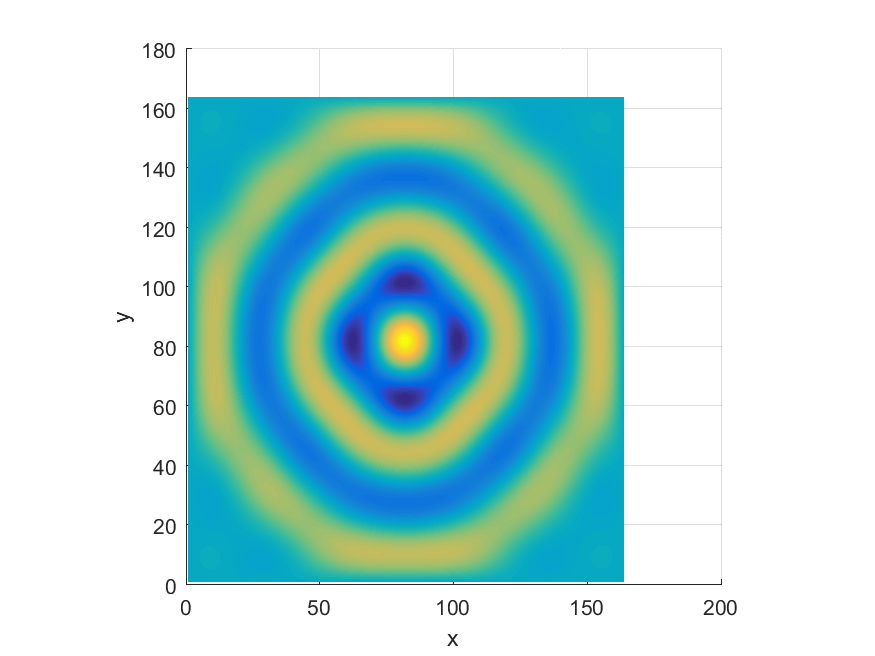
\includegraphics[width=6cm]{./Chapter_4/_Figs/Monopole001_5point_160Hz_L10m_8000Fs.png}
	\caption{T=0.015s}
\end{subfigure}
\begin{subfigure}{0.3 \textwidth}
	\centering
	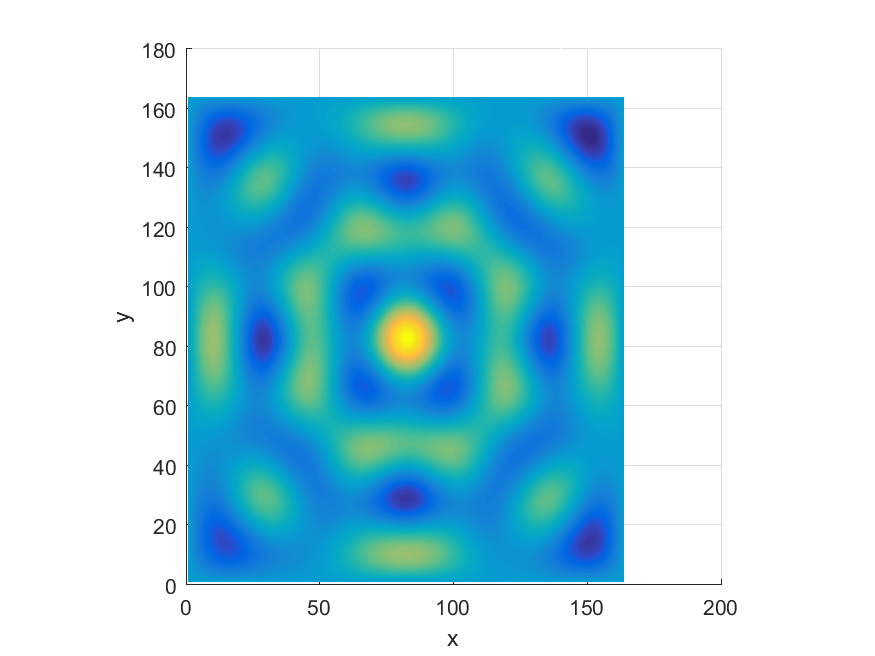
\includegraphics[width=6cm]{./Chapter_4/_Figs/Monopole05_5point_160Hz_L10m_8000Fs.png}
	\caption{T=0.5s}
\end{subfigure}
\begin{subfigure}{0.3 \textwidth}
	\centering
	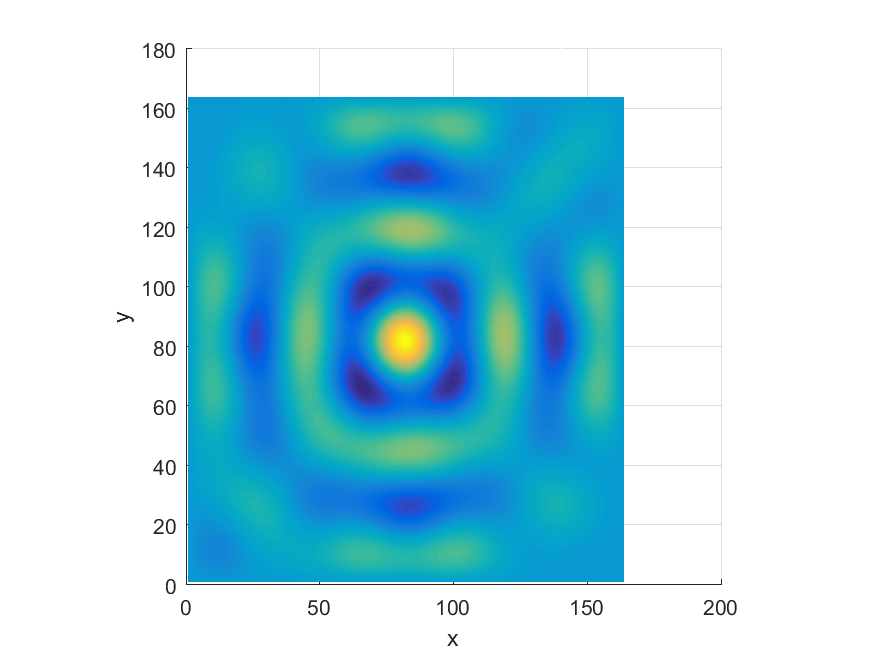
\includegraphics[width=6cm]{./Chapter_4/_Figs/Monopole1_5point_160Hz_L10m_8000Fs.png}
	\caption{T=1s}
\end{subfigure}
\caption{Radiation pattern of monopole approximation at different times T. Produced using 5 point sheme approximation to 2D wave equation}
\end{figure}


\section{Dipole}
\label{chapter4:sec2}
If we consider the combination of out phased monopoles situated in close proximity from one another, the radiation pattern that will be produced is that of a dipole. Moreover, if we reduce the distance between this monopoles to be sufficiently small with respect to the wavenumber, this combination of sources can be considered as a dipole source. Since we can consider a dipole source as a combination of two out phased monopoles, it important to understand the interference between this monopoles, the radiation pattern that a dipole will produce will not be omnidirectional. In fact, there are positions on the space where this combination of radiation will result on the absence of vibration and therefore sound. 
Before we see a clear example of such pattern, let us give a similar treatment to that of the monopole and so, we will only consider the dipole source once it is introduced into the wave equation. Therefore defining a dipole source as the driving force of the following equation we reach the defining expression for such source
\begin{equation}
\label{eqn:Dipole}
	u_{tt}=\gamma^{2}(\Delta u) + f(t)*D*\nabla(\delta(x-x_{s}),\delta(y-y_{s}))
\end{equation}
Since the radiation patterns are not omnidirectional, it is interesting to produce an approximation to the source that can vary its positioning in space and therefore have the possibility of rotation. In order to produce rotation, it is necessary to introduce the following rotation vector $\vec{r}=(cos(\theta),sin(\theta))$, which will multiply the dipole expression and produce a rotation given by the angle $\theta$.\\
Following the analysis of a monopole source, we can reach a similar approximation equation for the wave propagation as
\begin{equation}
\label{eqn:FD5dipo}
	\begin{aligned}
	u^{n+1}_{s,p}&=2u^{n}_{s,p}-u^{n-1}_{s,p}+\lamba^{2}(u^{n}_{s+1,p}+u^{n}_{s-1,p}+u^{n}_{s,p+1}+u^{n}_{s,p-1}-4u^{n}_{s,p}) \\
			&+ Q*f(t)*\vec{r}*\nabla(\frac{sin(\pi(x-x_{s}))}{\pi(x-x_{s})},\frac{sin(\pi(y-y_{s}))}{\pi(y-y_{s})})
	\end{aligned}
\end{equation}
Which produce the radiation patterns illustrated on Figure $\ref{figs:dipole}$ for the same parameters as the ones given for the monopole approximation.
\begin{figure}[h]
\begin{subfigure}{0.3 \textwidth}
	\centering
	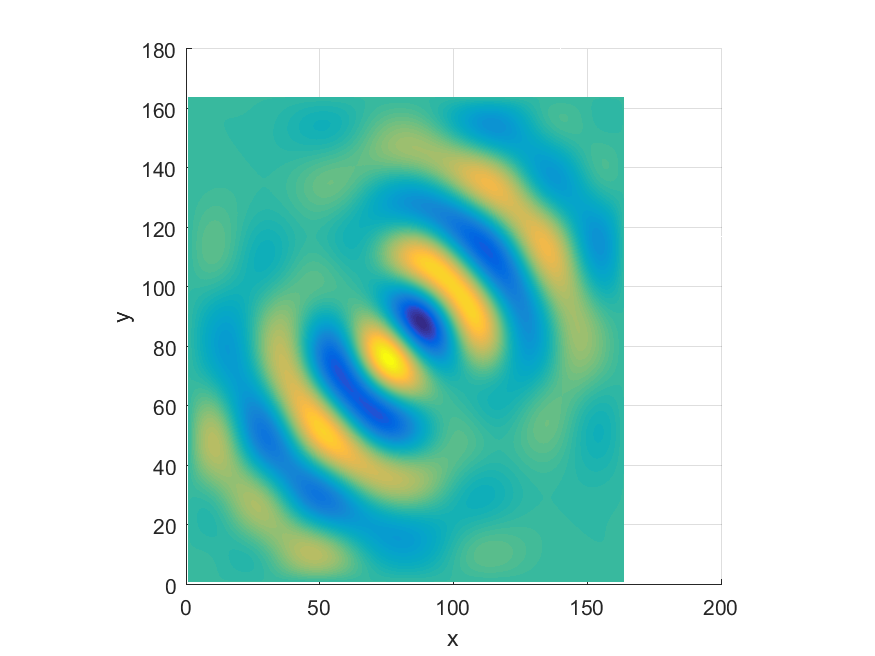
\includegraphics[width=6cm]{./Chapter_4/_Figs/Dipole001_5point_160Hz_L10m_8000Fs.png}
	\caption{T=0.015s}
\end{subfigure}
\begin{subfigure}{0.3 \textwidth}
	\centering
	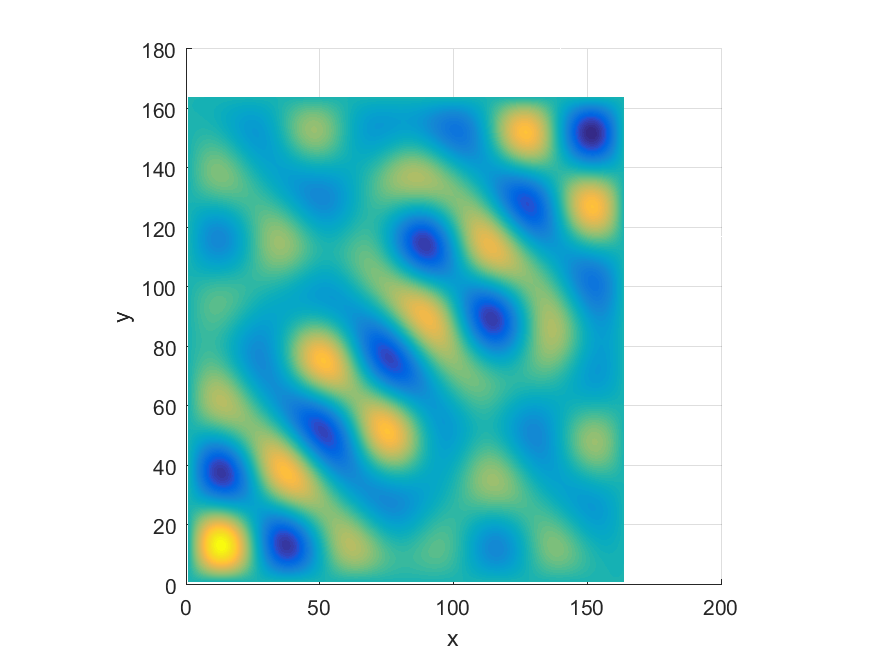
\includegraphics[width=6cm]{./Chapter_4/_Figs/Dipole05_5point_160Hz_L10m_8000Fs.png}
	\caption{T=0.5s}
\end{subfigure}
\begin{subfigure}{0.3 \textwidth}
	\centering
	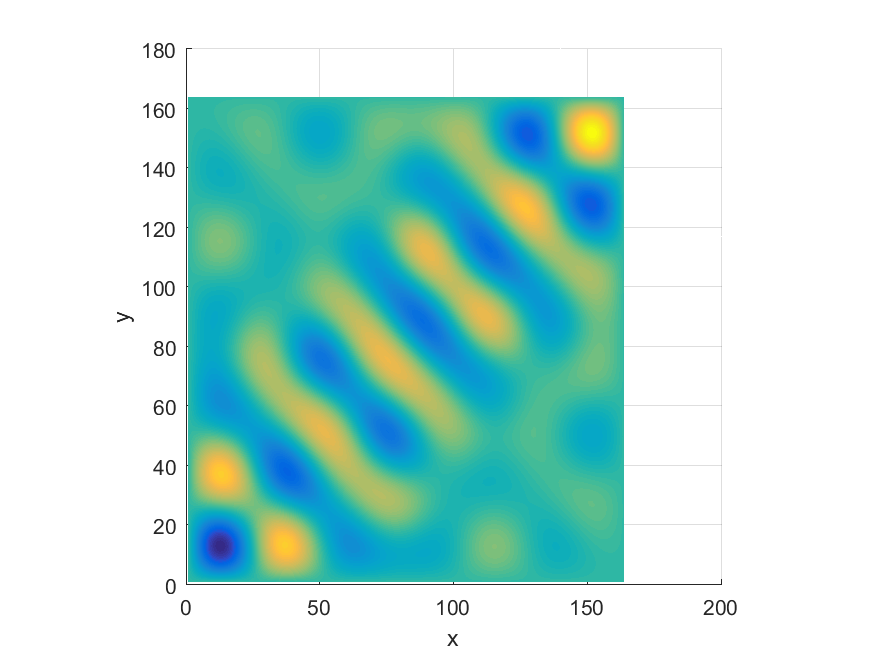
\includegraphics[width=6cm]{./Chapter_4/_Figs/Dipole1_5point_160Hz_L10m_8000Fs.png}
	\caption{T=1s}
\end{subfigure}
\label{figs:dipole}
\end{figure}

\section{Quadrupole}
\label{chapter4:sec3}
The most intuitive way to describe the radiation pattern produced by a quadrupole is to think of it as two dipoles out of phase at a small distance appart. Once again, if this distance is reduced considerably with respect to the wavenumber, this becomes a quadrupole source.\\ 
There are different combination of dipoles that can produce a quadrupole source. In this study, we will focus on two particular quadrupoles, $\textit{lateral}$ and $\textit{longitudinal}$. $\textit{Lateral}$ quadrupole consists on the combination of two perpendicular dipoles while $\texit{longitudinal}$ quadrupole will consists on the combination of two parallel dipoles.\\
Using the previous definition of dipole we can now define the quadrupole as
\begin{equation}
\label{eqn:Quadrupole}
	u_{tt}=\gamma^{2}(\Delta u) + f(t)*C*\nabla^{2}(\delta(x-x_{s}),\delta(y-y_{s}))
\end{equation}
Since the radiation patterns are not omnidirectional, it is interesting to produce an approximation to the source that can vary its positioning in space and therefore have the possibility of rotation. In order to produce rotation, it is necessary to introduce the following rotational matrices respectively for the longitudinal and lateral quadrupole as
\begin{equation}
	Q=\begin{bmatrix}
		cos(\theta)^2   & cos(\theta)sin(\theta)\\
		 cos(\theta)sine(\theta) & sin(\theta)^{2}
	\end{bmatrix}
	\ \ \ \ \
	Q_{x}=\begin{bmatrix}
		cos(\theta)sin(\theta)& 0.5(cos(\theta)^{2}-sin(\theta)^{2})\\
		 0.5(cos(\theta)^{2}-sin(\theta)^{2}) &  cos(\theta)sine(\theta) 
	\end{bmatrix}
\end{equation}  
Which will respectively multiply each particular quadrupole expression and produce a rotation given by the angle $\theta$.\\
Following the analysis of a monopole source, we can reach a similar approximation equation for the wave propagation driven by a lateral quadrupole as
\begin{equation}
\label{eqn:FD5dquadlat}
	\begin{aligned}
	u^{n+1}_{s,p}&=2u^{n}_{s,p}-u^{n-1}_{s,p}+\lamba^{2}(u^{n}_{s+1,p}+u^{n}_{s-1,p}+u^{n}_{s,p+1}+u^{n}_{s,p-1}-4u^{n}_{s,p}) \\
			&+ C*f(t)*Q*\nabla^{2}(\frac{sin(\pi(x-x_{s}))}{\pi(x-x_{s})},\frac{sin(\pi(y-y_{s}))}{\pi(y-y_{s})})
	\end{aligned}
\end{equation}
While the longitudinal quadrupole equation would be given by
\begin{equation}
\label{eqn:FD5dquadlat}
	\begin{aligned}
	u^{n+1}_{s,p}&=2u^{n}_{s,p}-u^{n-1}_{s,p}+\lamba^{2}(u^{n}_{s+1,p}+u^{n}_{s-1,p}+u^{n}_{s,p+1}+u^{n}_{s,p-1}-4u^{n}_{s,p}) \\
			&+ C*f(t)*Q_{x}*\nabla^{2}(\frac{sin(\pi(x-x_{s}))}{\pi(x-x_{s})},\frac{sin(\pi(y-y_{s}))}{\pi(y-y_{s})})
	\end{aligned}
\end{equation}
The radiation patterns produced by the lateral quadrupole are visulaized in Figure $\ref{figs:latquad}$ which are based on the same parameters as the two previous sources.
\begin{figure}[h]
\begin{subfigure}{0.3 \textwidth}
	\centering
	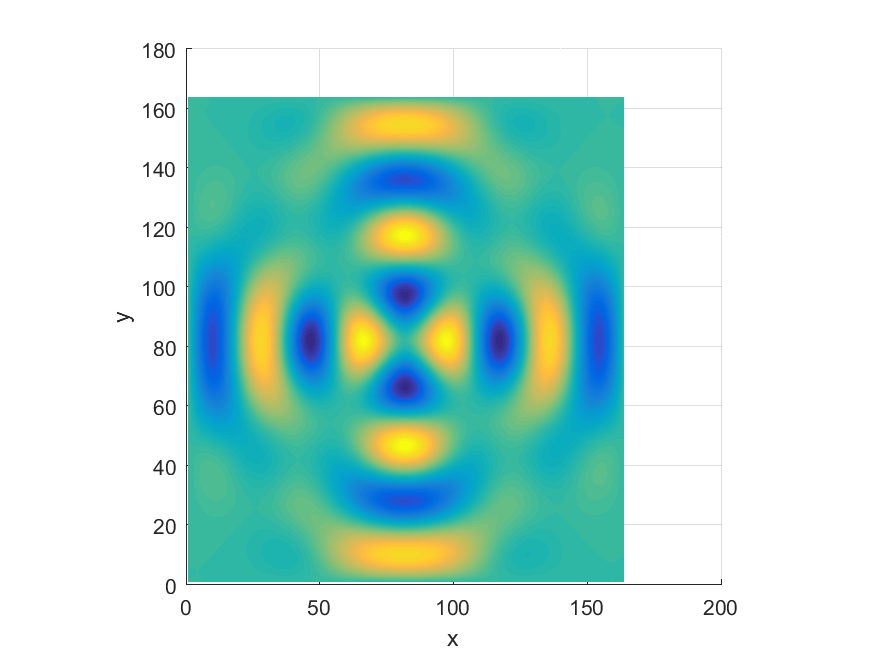
\includegraphics[width=6cm]{./Chapter_4/_Figs/Quadrupole_lateral_001_5point_160Hz_L10m_8000Fs.png}
	\caption{T=0.015s}
\end{subfigure}
\begin{subfigure}{0.3 \textwidth}
	\centering
	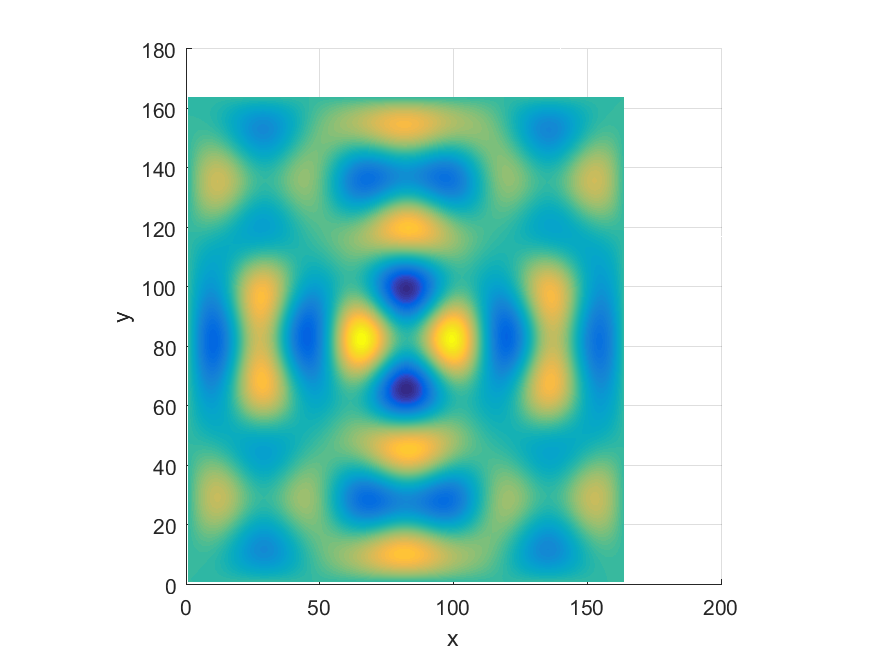
\includegraphics[width=6cm]{./Chapter_4/_Figs/Quadrupole05_lateral_5point_160Hz_L10m_8000Fs.png}
	\caption{T=0.3s}
\end{subfigure}
\begin{subfigure}{0.3 \textwidth}
	\centering
	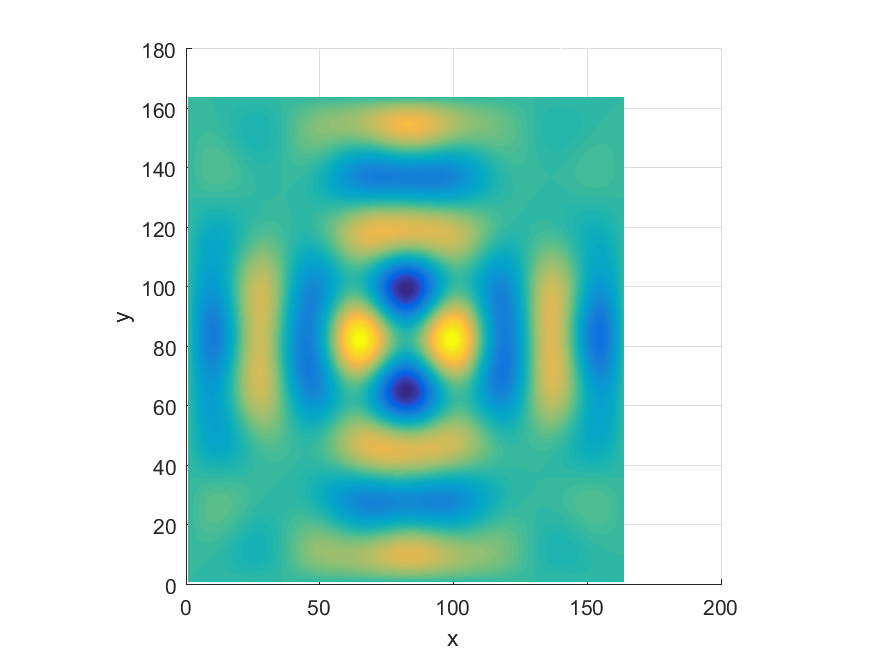
\includegraphics[width=6cm]{./Chapter_4/_Figs/Quadrupole1_lateral_5point_160Hz_L10m_8000Fs.png}
	\caption{T=1s}
\end{subfigure}
\label{figs:latquad}
\end{figure}


%%%%%%%%%%%% EDIT %%%%%%%%%%%%